\documentclass{beamer}
\usetheme{Madrid}       % Тема презентації
\usecolortheme{default} % Кольорова схема

\title{Презентація про мене}
\author{Бондар Наталія}      % Ваше ім'я
\institute{ВДПУ} % Назва навчального закладу
\date{\today}

\usepackage[utf8]{inputenc}
\usepackage[T2A]{fontenc}
\usepackage[ukrainian]{babel}
\usepackage{graphicx}   % для графіки

\begin{document}

% Титульний слайд
\frame{\titlepage}

% Зміст
\begin{frame}
\frametitle{Зміст}
\tableofcontents
\end{frame}

% Розділ: Вступ
\section{Вступ}
\begin{frame}
\frametitle{Вступ}
\begin{itemize}
    \item Спеціальність: математика
    \item Рік навчання: 2 курс
    \item Основні предмети: Математика, Інформатика, 
\end{itemize}
\end{frame}

% Розділ: Академічні досягнення
\section{Академічні досягнення}
\begin{frame}
\frametitle{Академічні досягнення}
\begin{itemize}
    \item Участь у шкільних олімпіадах з математики та фізики
    \item Сертифікати курсів з LaTeX та Python
    \item Проекти: створення презентацій та простих програм
\end{itemize}
\end{frame}

\section{Навчальні інтереси}
\begin{frame}{Навчальні інтереси}
    \begin{columns}[c] % Вирівнювання по центру по вертикалі
        
        % Ліва колонка
        \begin{column}{0.6\textwidth}
            \begin{itemize}
                \item вивчення геометрії
                \item вибіркові предмети (гейміфікація в освіті; тренінг по розвитку стресостійкості)
                \item Робота з графікою та LaTeX
            \end{itemize}
        \end{column}

        % Права колонка
        \begin{column}{0.3\textwidth}
            \centering
            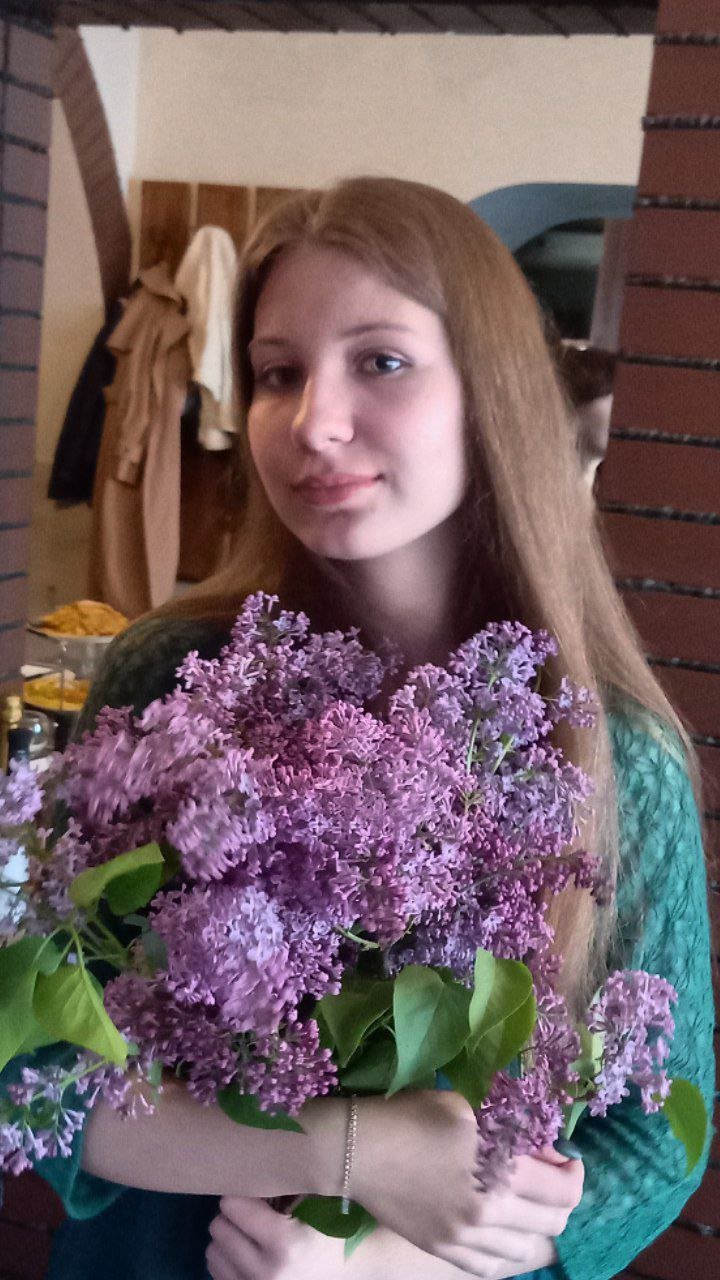
\includegraphics[width=\textwidth]{foto1.png}
        \end{column}
        
    \end{columns}
\end{frame}


\section{Коротко про мене}
\begin{frame}
\frametitle{Коротко про мене}
\begin{itemize}
    \item Вік: 18р
    \item Місце проживання: смт. Сутиски
    \item де навчалась: Суитисківський ліцей
    \item брати/сестри: єдина дитина в сім'ї
\end{itemize}
\centering
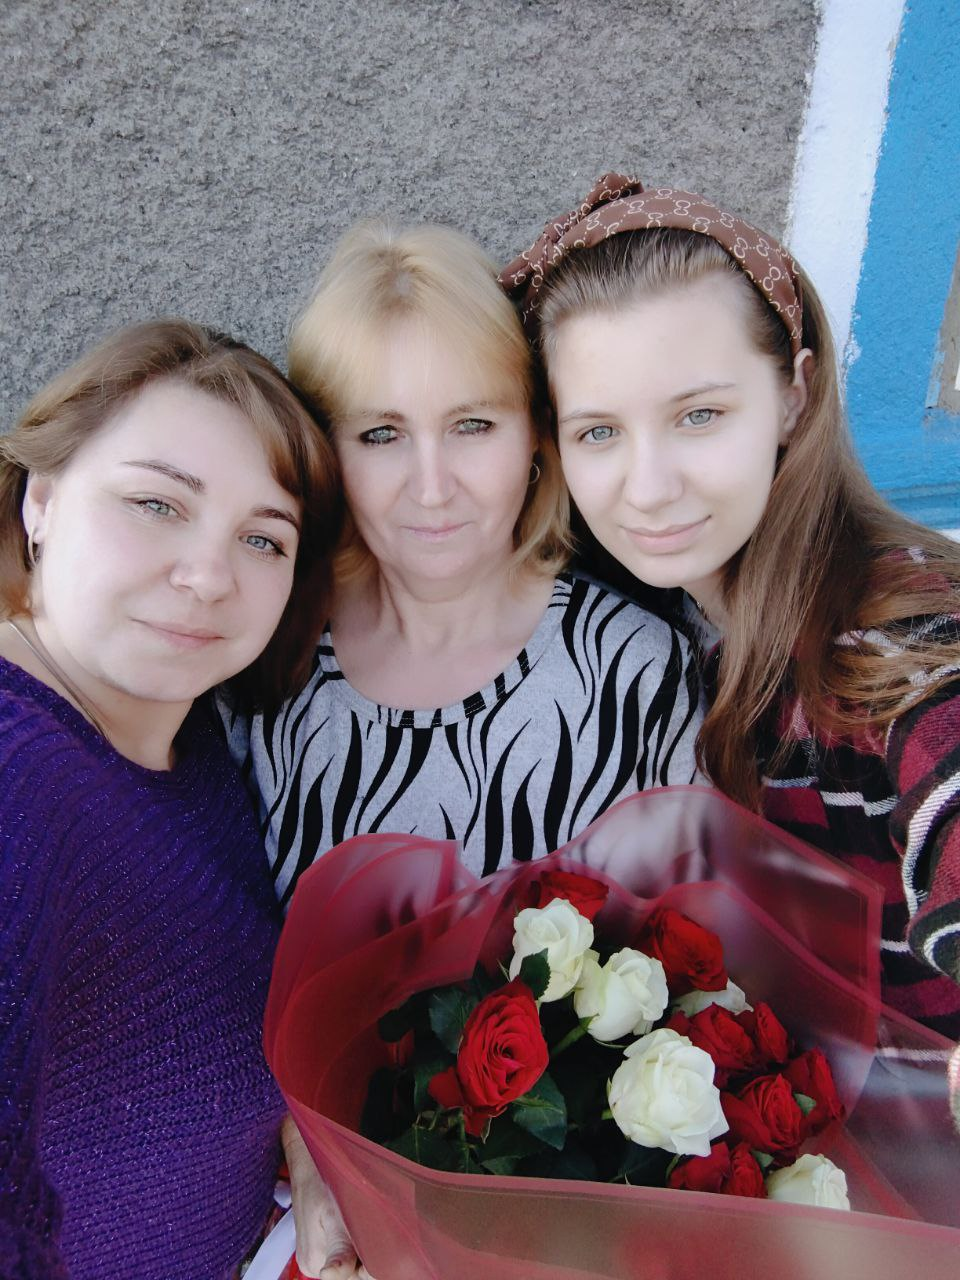
\includegraphics[width=0.2\textwidth]{foto2.png} % Вставити зображення

\vspace{0.5cm} % вертикальний відступ між зображенням та списком
\end{frame}

\section{Моє хоббі}
\begin{frame}
\frametitle{Моє хоббі}
\begin{itemize}
    \item картини по номерах; алмазні мозайки
    \item вироби з бісеру
    \item ручні вироби 
\end{itemize}
\end{frame}

% Розділ: Висновок
\section{Висновок}
\begin{frame}
\frametitle{Висновок}
Презентація демонструє основні академічні досягнення, навчальні інтереси та проєктну діяльність студента.
\end{frame}

\end{document}